\section[日志输出器]{日志输出器}\label{sec:日志输出器}

\subsection[日志的结构]{日志的结构}\label{subsec:日志的结构}

日志类的UML图如下所示

\begin{figure}[h]
    \label{fig:日志结构}
    \centering
    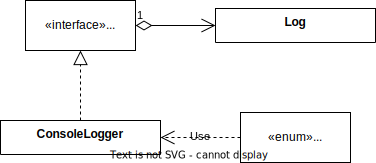
\includegraphics{img/日志类结构.svg}
    \caption{日志类的UML图}
\end{figure}

其中\codeline{ConsoleLogger}是内核中的一个日志输出器的实现。我们自己实现的日志输出器会替代它的位置。在实际使用日志时调用的是\codeline{Log}类,它包含一个\codeline{Logger},因此我们的日志输出器要实现\codeline{Logger}接口。\codeline{LogLevel}是日志的等级,如下表所示。

\begin{longtable}{p{2cm}|p{9cm}}
    日志等级 & 含义 \\
    \hline
    v & 冗长信息,指一般不需要过多关注,但是需要在日志中输出的信息\\
    \hline
    d & debug信息,建议在单元测试使用\\
    \hline
    i & 一般信息\\
    \hline
    w & 警告信息,比如传入的参数不规范,可能会导致报错时使用\\
    \hline
    e & 错误信息
\end{longtable}

\subsection[编写日志输出器]{编写日志输出器}\label{subsec:编写日志输出器}

编写日志输出器,首先要继承\codeline{Logger接口}并实现其中的所有方法。

\begin{lstlisting}[style=Java, caption={Logger初始布局},label={lst:Logger初始布局}]
public class MyLogger implements Logger
{
    @Override
    public void v(String tag, String message)
    {

    }

    @Override
    public void v(String tag, String message, Throwable throwable)
    {

    }
    // 其它方法
    // ...
}
\end{lstlisting}

每个方法的方法名都对应了日志等级。参数\codeline{String tag}是日志的标签,其作用是标记出给出日志的类。参数\codeline{String message}是日志的内容。参数\codeline{Throwable throwable}用于将报错的信息打印出来以便定位错误。这个参数是可选的,因为显然不一定所有日志都有报错信息。

这里给出\codeline{ConsoleLogger}的部分源码以供参考。

\begin{lstlisting}[style=Java, caption={ConsoleLogger源码},label={lst:ConsoleLogger源码}]
package com.potato.Log;

/**
 * ConsoleLogOutput是将日志输出至终端的一个实现
 */
public class ConsoleLogger implements Logger
{
    /**
     * 一般日志输出至标准输出流
     *
     * @param tag       用于分辨日志来源,可以设置为类名
     * @param message   日志信息
     * @param throwable 提供给日志的报错
     */
    private void normalPrintln(String tag, String message, Throwable throwable, LogLevel logLevel)
    {
        if (throwable != null)
        {
            System.out.printf("TAG:%s\t%s:%s\tTHROWABLE:%s%n", tag, logLevel, message, throwable);
        }
        else
        {
            System.out.printf("TAG:%s\t%s:%s%n", tag, logLevel, message);
        }
    }

    // 省略errorPrintln()的代码,它就是把normalPrintln()的out换成的err
    // 省略v()和d()的代码

    /**
     * 输出一般的信息
     *
     * @param tag     用于分辨日志来源,可以设置为类名
     * @param message 日志信息
     */
    @Override
    public void i(String tag, String message)
    {
        normalPrintln(tag, message, null, LogLevel.INFO);
    }

    /**
     * 输出一般的信息
     *
     * @param tag       用于分辨日志来源,可以设置为类名
     * @param message   日志信息
     * @param throwable 提供给日志的报错
     */
    @Override
    public void i(String tag, String message, Throwable throwable)
    {
        normalPrintln(tag, message, throwable, LogLevel.INFO);
    }

    // 省略w()的代码

    /**
     * 输出错误信息
     *
     * @param tag     用于分辨日志来源,可以设置为类名
     * @param message 日志信息
     */
    @Override
    public void e(String tag, String message)
    {
        errorPrintln(tag, message, null, LogLevel.ERROR);
    }

    /**
     * 输出错误信息
     *
     * @param tag       用于分辨日志来源,可以设置为类名
     * @param message   日志信息
     * @param throwable 提供给日志的报错
     */
    @Override
    public void e(String tag, String message, Throwable throwable)
    {
        errorPrintln(tag, message, throwable, LogLevel.ERROR);
    }
}

\end{lstlisting}

在编写完日志输出器后,在\codeline{Config}初始化时将\codeline{Logger logger}参数设置为自定义的日志输出器即可。

\begin{lstlisting}[style=Java, caption={设置日志输出器},label={lst:设置日志输出器}]
File configFile = // 配置文件
Config.initial(configFile, null, null, null, new MyLogger());
\end{lstlisting}

这里给出一个调用\codeline{Log}的实例:

\begin{lstlisting}[style=Java, caption={Log调用实例},label={lst:Log调用实例}]
catch (NoSuchMethodException e)
{
    Log.e(Config.class.toString(), "未找到对应解析器或管理器", e);
    throw new RuntimeException(e);
}
\end{lstlisting}
